\section{Introducción}
  
\subsection*{Contexto}
% Una subsection* crea un nuevo "grupo de puntos"

\frame{
	\ifdebug
	\frametitle{Descripción del problema\hfill{\color{red} \emph{A}}}

	\else
		\frametitle{Descripción del problema}
	\fi

	\textbf{Objetivo}
	\vspace{0.25cm}
	\begin{center}
		``Diseñar, ensamblar y programar una planta móvil de control de
		  nivel, utilizando transmisores de señal, controladores y
		  actuadores
		  industriales disponibles en el mercado''
	\end{center}
	\textbf{Es decir, algo así}...
	\begin{center}
	  %\vspace{0.25cm}
	  \begin{figure}[h!]
	  \centering
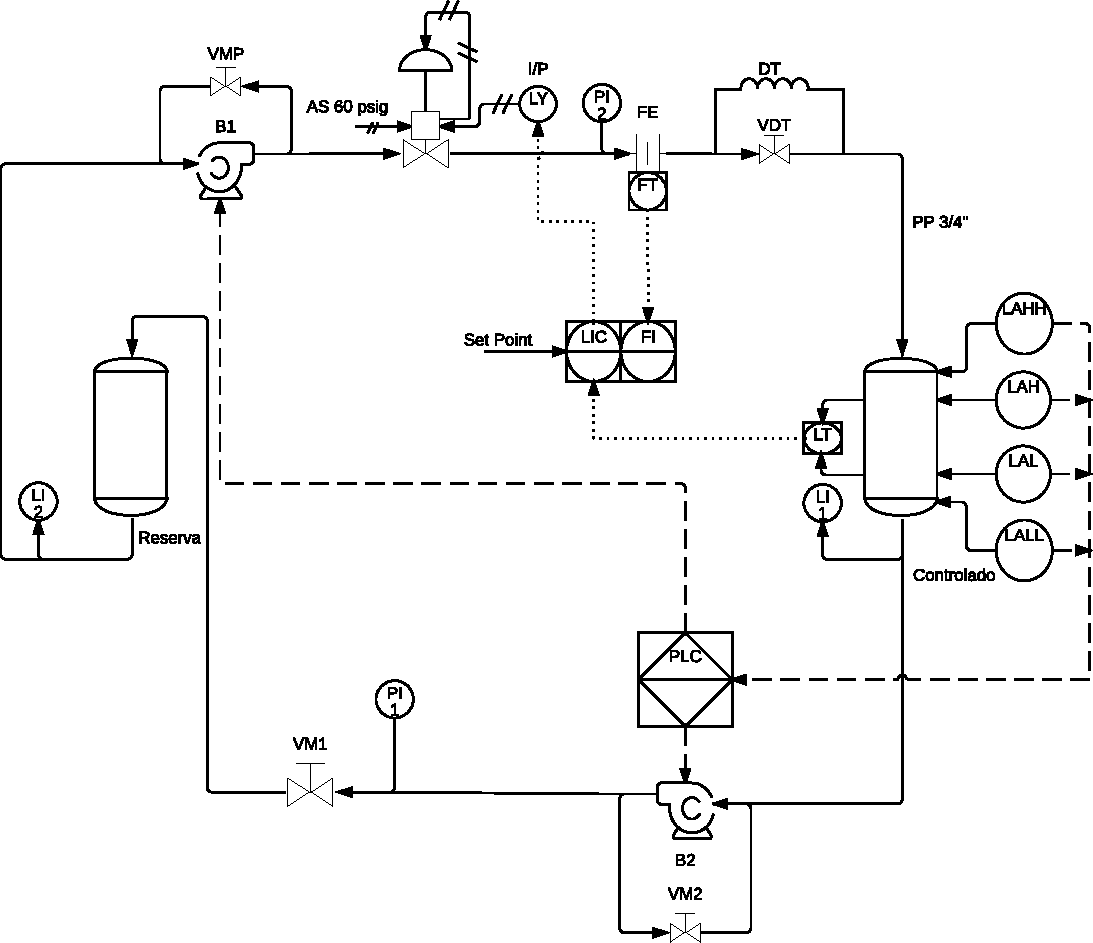
\includegraphics[width=.49\textwidth]
{Sections/2-DisenoEnsamblado/Images/pyid60-1.pdf}
	  \end{figure}
	\end{center}
}

\frame{
	\ifdebug
	\frametitle{Solución propuesta - Especificaciones\hfill{\color{red}
\emph{A}}}
	\else
	\frametitle{Solución propuesta - Especificaciones}
	\fi
	
	\begin{columns}[t]
		\begin{column}{0.45\textwidth}
		\textbf{Solución Propuesta}...

		  \begin{center}
		    \begin{figure}[h!]
		      \centering
			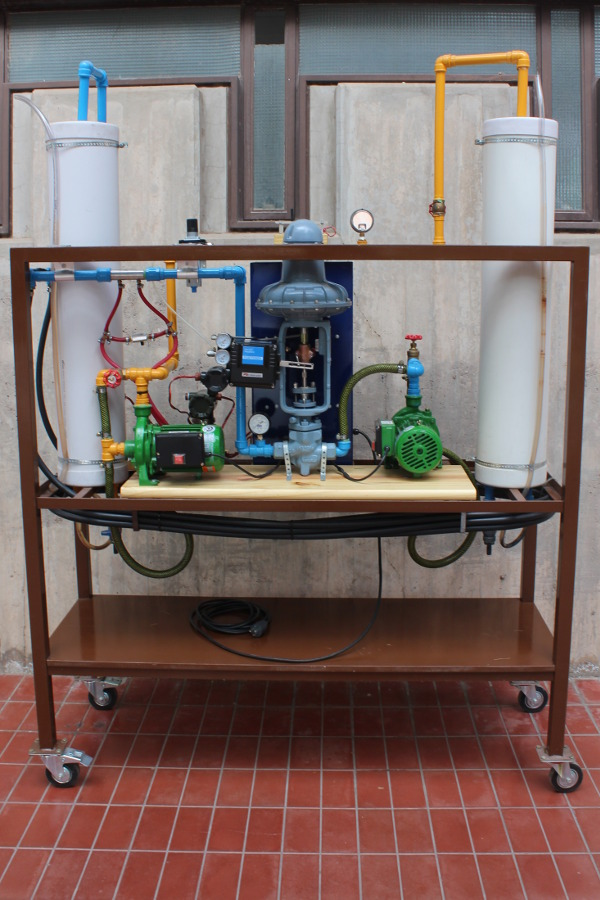
\includegraphics[width=.9\textwidth]
			 {Sections/1-Introduccion/images/IMG_5123.jpeg}
			\end{figure}
		   \end{center}
		\end{column}
		\begin{column}{0.45\textwidth}
		\textbf{Especificaciones}...

		\vspace{.5cm}
		La planta debe:
			\begin{enumerate}
				\item Representar un ambiente industrial
				\begin{itemize}
				 \item Procesos
				 \item Elementos
				\end{itemize}

				\item Cumplir un objetivo pedagógico
				\begin{itemize}
		\item Verificar el funcionamiento del conjunto
		\item Documentar: manual del usuario de la planta
				 \end{itemize}

		\item Tener un costo inferior a una solución llave en mano
			\end{enumerate}
		\end{column}
	\end{columns}
}

\frame{
	\ifdebug
	\frametitle{Análisis económico\hfill{\color{red} \emph{A}}}
	\else
	\frametitle{Análisis económico}
	\fi

	\begin{columns}
	  \centering
	 \begin{column}{0.3\textwidth}
	    \centering
	    \textbf{Cuál es el costo?}
	 \end{column}
	 
	 \begin{column}{0.3\textwidth}
	    \textbf{Plantas Similares:}
	    \begin{itemize}
	     \item Llave en mano.
	     \item Puerto de Bs.As.
	    \end{itemize}
	 \end{column}

	 \begin{column}{0.3\textwidth}
	    \begin{ukblock}
		\centering
		\textbf{16200 USD}
	    \end{ukblock}
	    \begin{itblock}
		\centering
		\textbf{28400 EUR}
	    \end{itblock}
	 \end{column}
	\end{columns}

	
	\vspace{-0.5cm}
	\begin{center}
%	 Las partes constitutivas de ambas plantas son elementos industriales
	 \end{center}
	\textbf{Donaciones:}
	\vspace{0.2cm}
	\begin{columns}[T]
	
	 \begin{column}{0.3\textwidth}
	    \begin{techintblock}
		\centering
		\textbf{23200 ARS}
	    \end{techintblock}
	    \footnotesize
	    \begin{itemize}
	     \item Electrobombas
	     \item PLC+PS+Mod. Analógico
	     \item DP Cell
	     \item Válvula de control
	    \end{itemize}
	 \end{column}
	 
	 \begin{column}{0.3\textwidth}
	    \begin{fingblock}
		\centering
		\textbf{8700 ARS}
	    \end{fingblock}
	    \footnotesize
	     \begin{itemize}
	      \item Estructura
	      \item Tuberías y Acc.
	      \item Material Eléctrico
	      \item Manómetros.
	     \end{itemize}
	 \end{column}

	 \begin{column}{0.3\textwidth}
	    \begin{puglesiblock}
		\centering
		\textbf{450 ARS}
	    \end{puglesiblock}
	    \footnotesize
	    \begin{itemize}
	     \item Placa Orificio
	    \end{itemize}

	 \end{column}

	\end{columns}
	
}

\begin{frame}
	\ifdebug
	\frametitle{Tareas Realizadas\hfill{\color{red} \emph{A}}}
	\else
	\frametitle{Tareas Realizadas}
	\fi
	
	 \centering
	  La construcción de la planta implica una serie de etapas que deben 
realizarse de manera ordenada
	 
	 \begin{columns}
	  \begin{column}{0.5\textwidth}
	   \begin{enumerate}
	    \item Planificación y diseño preliminar
	    \item Construcción de la planta
	    \item Programación del PLC
	   \end{enumerate}
	    \begin{figure}[h!]
	  \centering
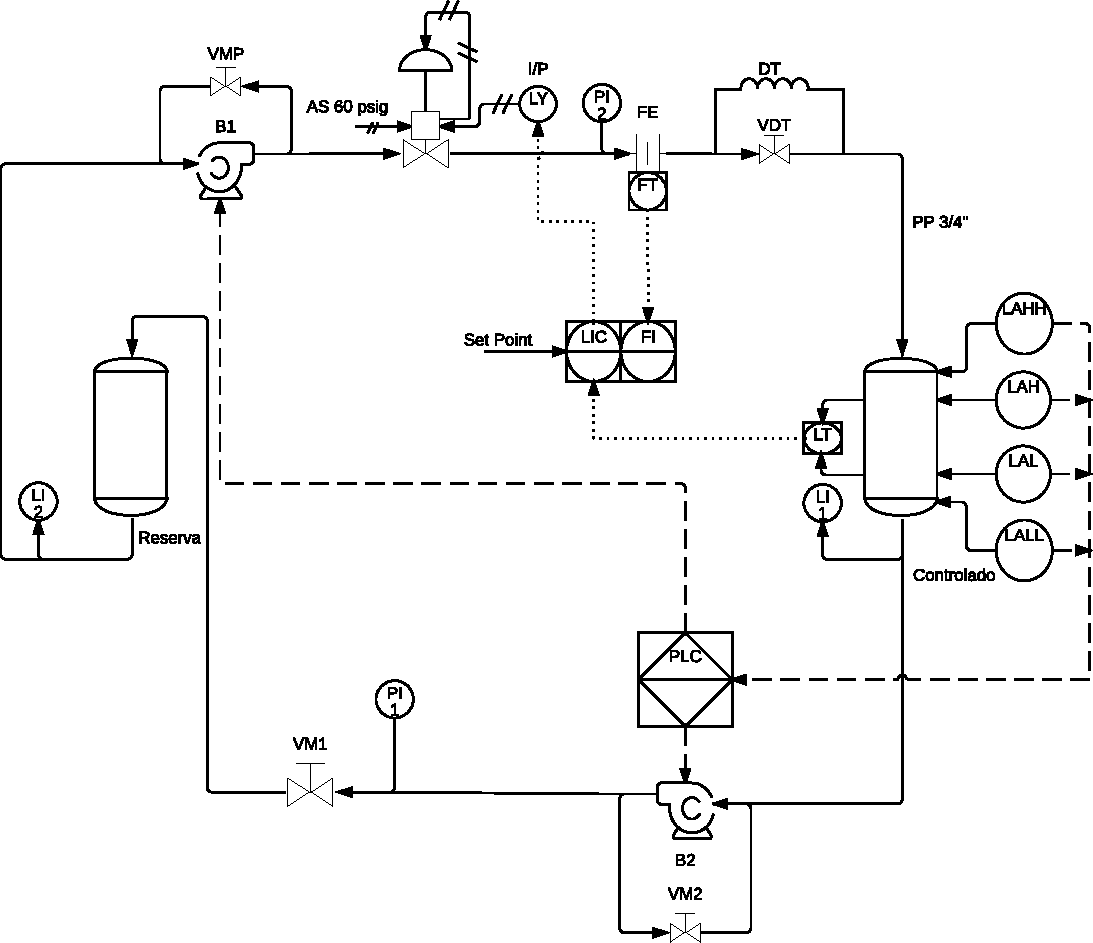
\includegraphics[width=.8\textwidth]
{Sections/2-DisenoEnsamblado/Images/pyid60-1.pdf}
	  \end{figure}
	  \end{column}
	  
	  \begin{column}{0.5\textwidth}
	  \begin{enumerate}
	    \item Programación SCADA
	    \item Pruebas de funcionamiento
	    \item Documentación
	   \end{enumerate}
	\begin{figure}[!ht]
	\centering
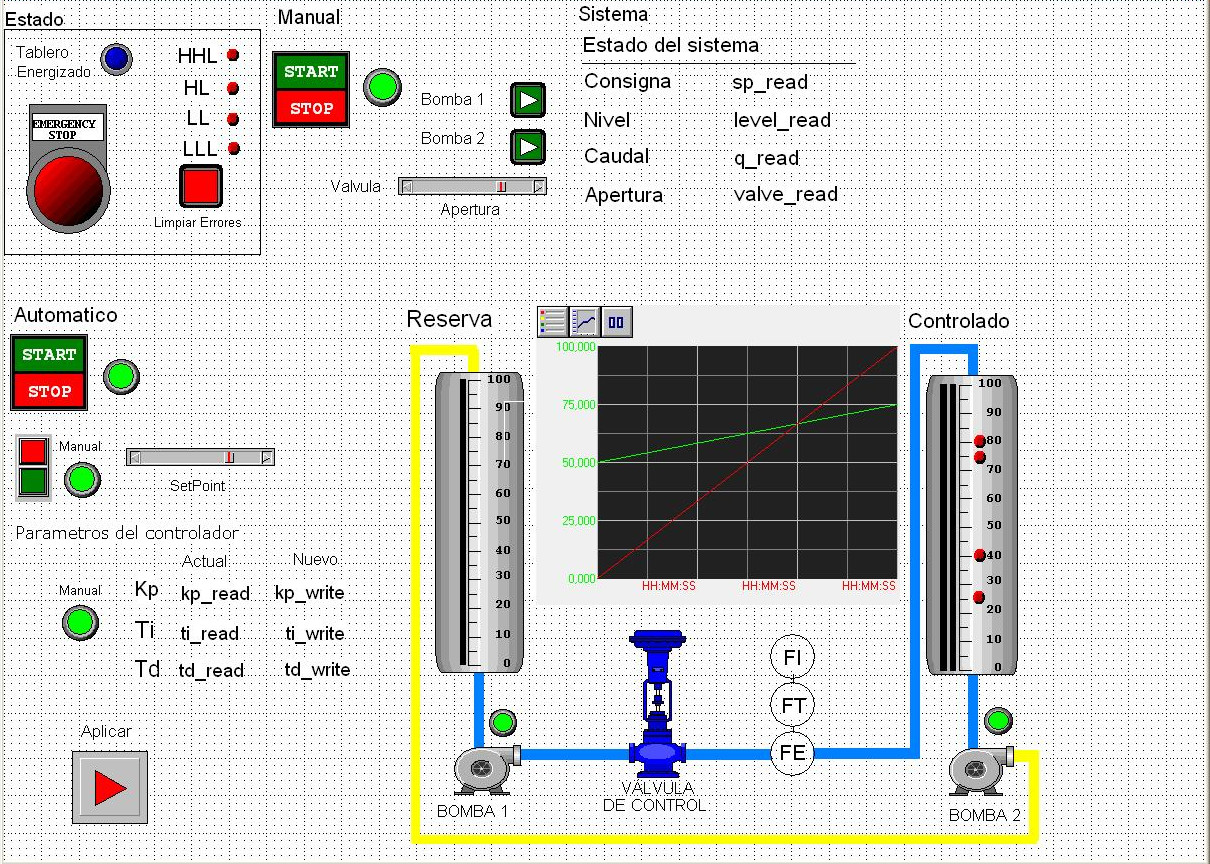
\includegraphics[width=0.8\textwidth]
{../Informe/Cap5-SCADA/images/hmiScada.jpeg}
	\end{figure}	  
	  \end{column}
	 \end{columns}

	 


\end{frame}

\begin{frame}
	\ifdebug
	\frametitle{Outline\hfill{\color{red} \emph{A}}}
	\else
	\frametitle{Outline}
	\fi

    \tableofcontents
\end{frame}
